\begin{figure}[p]
\centering
\begin{tikzpicture}[x=1cm,y=1cm,>=Stealth,font=\small]
\filldraw[draw=inkblue,fill=inkblue!65] (1,11.8) rectangle (9.6,12);
\filldraw[draw=inkblue,fill=red!90] (9.6,11.65) rectangle (12.2,12.1);
\node[text=white] at (10.9,11.87) {AAAAAAA};
\draw[green!70!black,very thick,->] (5.8,11.6)--(5.8,10.8);
\node at (2.9,11.2) {打断};
\node[anchor=west] at (10.3,10.8) {200--300 bp};
\foreach \x/\y in {1.4/10.7,2.2/10.95,3.7/10.7,4.2/10.95,6.5/10.8,7/11.05,8.4/10.8,8.9/11.05}
 \filldraw[draw=inkblue,fill=inkblue!65] (\x,\y) rectangle ++(1,.12);
\node at (3.2,10.2) {RNA 片段};
\foreach \x in {1,4.2,7.4}{
 \fill[red!90] (\x,9.5) rectangle ++(.8,.15);
 \filldraw[draw=inkblue,fill=inkblue!65] (\x+.8,9.5) rectangle ++(1,.15);
 \fill[red!90] (\x+1.8,9.5) rectangle ++(.8,.15);
 \fill[red!90] (\x,9.25) rectangle ++(.8,.15);
 \filldraw[draw=inkblue,fill=inkblue!65] (\x+.8,9.25) rectangle ++(1,.15);
 \fill[red!90] (\x+1.8,9.25) rectangle ++(.8,.15);
}
\node[text=red,anchor=east] at (.9,9.3) {接头};
\draw[green!65!black,->] (.45,9.5)--(1,9.6);
\node[anchor=west] at (10.25,9.45) {构建测序文库};
\node[anchor=east] at (.7,8) {基因};
\foreach \x in {1,4.5,8.3} \fill[green!65!black] (\x,7.95) rectangle ++(2.5,.2);
\foreach \x/\y in {1.2/7.3,1.4/7.05,2.1/7.55,2.5/6.8,3/7.1,4.45/7.55,4.6/7.15,5.35/6.9,5.8/7.5,6/7.1,8.4/7.15,8.9/7.5,9/6.9,10/7.1}
 \filldraw[draw=inkblue,fill=inkblue!65] (\x,\y) rectangle ++(1,.12);
\draw[green!65!black,dashed] (3.1,7.6)--(4.45,7.6);
\draw[green!65!black,dashed] (4,7.15)--(4.6,7.2);
\draw[green!65!black,dashed] (7,7.15)--(8.4,7.2);
\node[anchor=west] at (11.1,7.35) {剪接感知比对};
\node[anchor=east] at (.7,6.1) {基因组};
\fill[magenta!65] (1,6) rectangle (10.8,6.2);
\node[anchor=south west,inner sep=0] at (1,.0) {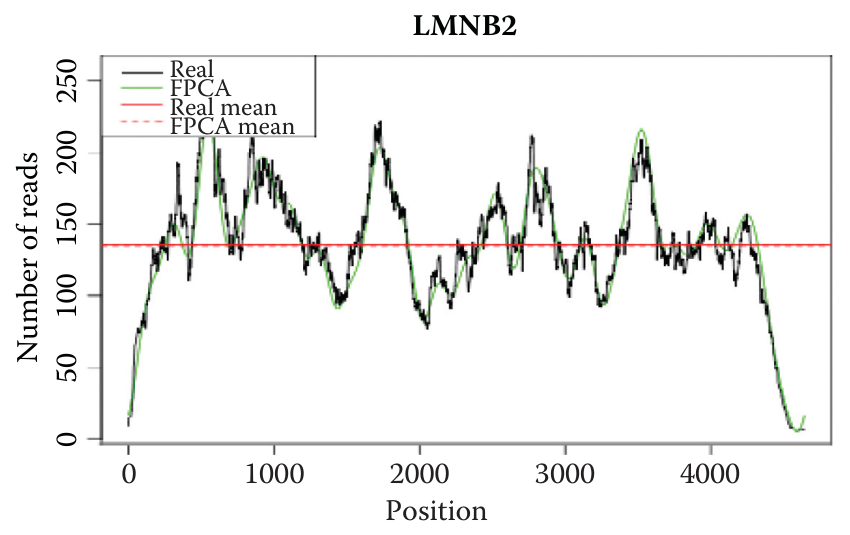
\includegraphics[width=9.4cm]{figures/ch04a_fig04_data.png}};
\node[anchor=west] at (10.7,3.2) {RNA 表达水平};
\fill[white] (5.224254595588236,0.06083399155560662) rectangle (6.4288921616498165,0.44789281508501844);
\node[font=\scriptsize,rotate=0,inner sep=0] at (5.826573378619026,0.25436340332031254) {位置};
\fill[white] (1.1239476336310892,1.876407434800092) rectangle (1.5220652806899126,4.262682387408089);
\node[font=\scriptsize,rotate=90,inner sep=0] at (1.323006457160501,3.0695449111040904) {读段数};
\filldraw[fill=white,draw=gray] (2.072705882352942,4.25764705882353) rectangle (4.621764705882353,5.3635294117647065);
\draw[black,solid,thin] (2.192705882352942,5.233529411764707)--(2.572705882352942,5.233529411764707);
\node[font=\tiny,anchor=west,inner sep=0] at (2.6427058823529417,5.233529411764707) {观测};
\draw[green!65!black,solid,thin] (2.192705882352942,4.993529411764706)--(2.572705882352942,4.993529411764706);
\node[font=\tiny,anchor=west,inner sep=0] at (2.6427058823529417,4.993529411764706) {FPCA};
\draw[red,solid,thin] (2.192705882352942,4.753529411764706)--(2.572705882352942,4.753529411764706);
\node[font=\tiny,anchor=west,inner sep=0] at (2.6427058823529417,4.753529411764706) {观测均值};
\draw[red,dashed,thin] (2.192705882352942,4.513529411764707)--(2.572705882352942,4.513529411764707);
\node[font=\tiny,anchor=west,inner sep=0] at (2.6427058823529417,4.513529411764707) {FPCA均值};
\end{tikzpicture}
\origfig{4}{RNA-seq 表达谱分析。}
\label{fig:ch04a-04}
\end{figure}
